% Don't touch this %%%%%%%%%%%%%%%%%%%%%%%%%%%%%%%%%%%%%%%%%%%
\documentclass[12pt]{article}
\usepackage{fullpage}
\usepackage[left=1in,top=1in,right=1in,bottom=1in,headheight=3ex,headsep=3ex]{geometry}
\usepackage{graphicx}
\usepackage{float}
\usepackage{array}


\newcommand{\blankline}{\quad\pagebreak[2]}
%%%%%%%%%%%%%%%%%%%%%%%%%%%%%%%%%%%%%%%%%%%%%%%%%%%%%%%%%%%%%%

% Modify Course title, instructor name, semester here %%%%%%%%

\title{PHY250 - Fall 2021: Fluids}
\author{}
\date{}

%%%%%%%%%%%%%%%%%%%%%%%%%%%%%%%%%%%%%%%%%%%%%%%%%%%%%%%%%%%%%%

% Don't touch this %%%%%%%%%%%%%%%%%%%%%%%%%%%%%%%%%%%%%%%%%%%
\usepackage[sc]{mathpazo}
%\linespread{1.05} % Palatino needs more leading (space between lines)
\usepackage[T1]{fontenc}
\usepackage[mmddyyyy]{datetime}% http://ctan.org/pkg/datetime
\usepackage{advdate}% http://ctan.org/pkg/advdate
\newdateformat{syldate}{\twodigit{\THEMONTH}/\twodigit{\THEDAY}}
\newsavebox{\MONDAY}\savebox{\MONDAY}{Mon}% Mon
\newcommand{\week}[1]{%
%  \cleardate{mydate}% Clear date
% \newdate{mydate}{\the\day}{\the\month}{\the\year}% Store date
  \paragraph*{\kern-2ex\quad #1, \syldate{\today} - \AdvanceDate[4]\syldate{\today}:}% Set heading  \quad #1
%  \setbox1=\hbox{\shortdayofweekname{\getdateday{mydate}}{\getdatemonth{mydate}}{\getdateyear{mydate}}}%
  \ifdim\wd1=\wd\MONDAY
    \AdvanceDate[7]
  \else
    \AdvanceDate[7]
  \fi%
}
%\usepackage{setspace}
\usepackage{multicol}
%\usepackage{indentfirst}
\usepackage{fancyhdr,lastpage}
\usepackage{url}
\pagestyle{fancy}
\usepackage{hyperref}
\usepackage{lastpage}
\usepackage{amsmath}
\usepackage{layout}

\lhead{}
\chead{}
%%%%%%%%%%%%%%%%%%%%%%%%%%%%%%%%%%%%%%%%%%%%%%%%%%%%%%%%%%%%%%

% Modify header here %%%%%%%%%%%%%%%%%%%%%%%%%%%%%%%%%%%%%%%%%
%\rhead{\footnotesize Text in header}

%%%%%%%%%%%%%%%%%%%%%%%%%%%%%%%%%%%%%%%%%%%%%%%%%%%%%%%%%%%%%%
% Don't touch this %%%%%%%%%%%%%%%%%%%%%%%%%%%%%%%%%%%%%%%%%%%
\lfoot{}
\cfoot{\small \thepage/\pageref*{LastPage}}
\rfoot{}

\usepackage{array, xcolor}
\usepackage{color,hyperref}
\definecolor{clemsonorange}{HTML}{EA6A20}
\hypersetup{colorlinks,breaklinks,linkcolor=clemsonorange,urlcolor=clemsonorange,anchorcolor=clemsonorange,citecolor=black}

\begin{document}

\maketitle




% First Section %%%%%%%%%%%%%%%%%%%%%%%%%%%%%%%%%%%%%%%%%%%%


\newcounter{example}
\setcounter{example}{1}

\section*{Exercise \theexample}

The surface of the water in a storage tank is 30 m above a water faucet in the kitchen of a house. Calculate the difference
in water pressure between the faucet and the surface of the water in the tank.
\vspace{5mm}

 \begin{figure}[h!]
  \begin{center}
    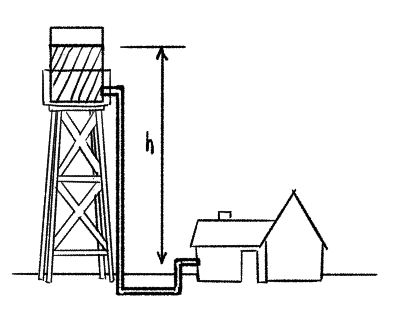
\includegraphics[height=2.in]{images/example1.jpg}
    \caption{Exercise \theexample }
    \label{1}
  \end{center}
\end{figure}

% Second Section %%%%%%%%%%%%%%%%%%%%%%%%%%%%%%%%%%%%%%%%%%%%
\stepcounter{example}

\section*{Exercise \theexample}

Force on aquarium window. Calculate the force due to water pressure exerted on a 1.0 m X 3.0 m aquarium viewing window whose top
edge is 1.0 m below the water surface

\vspace{5mm}


\begin{figure}[h!]
  \begin{center}
    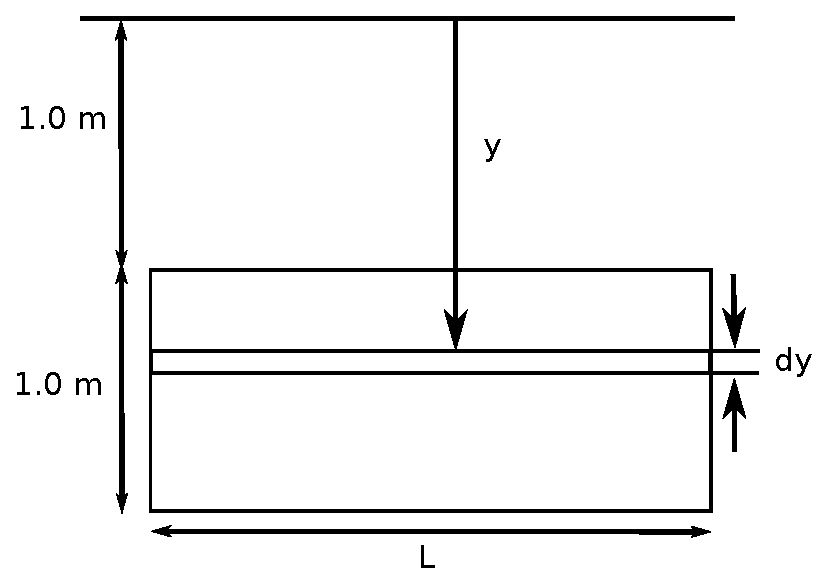
\includegraphics[height=2.in]{images/example2.eps}
    \caption{Exercise \theexample }
    \label{2}
  \end{center}
\end{figure}

% Third Section %%%%%%%%%%%%%%%%%%%%%%%%%%%%%%%%%%%%%%%%%%%%
\stepcounter{example}

\section*{Exercise \theexample}



At what elevation is the air pressure equal to half the pressure atsea level?


\stepcounter{example}

\section*{Exercise \theexample}


A U-shaped
tube with a horizontal portion of
length $\ell$ contains
a liquid. What is the difference
in height between the liquid
columns in the vertical arms (a)
if the tube has an acceleration a
toward the right and (b) if the
tube is mounted on a horizontal
turntable rotating with an angular speed $\omega$with one of the vertical
arms on the axis of rotation? (c) Explain why the difference in
height does not depend on the density of the liquid or on the crosssectional
area of the tube. Would it be the same if the vertical tubes
did not have equal cross-sectional areas? Would it be the same if the
horizontal portion were tapered from one end to the other? Explain.

\begin{figure}[h!]
  \begin{center}
  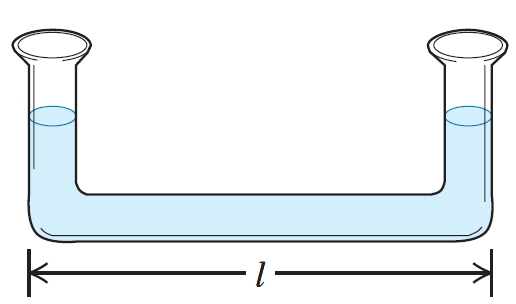
\includegraphics[height=1.3in]{images/example_12.85.jpg}
  \caption{Exercise \theexample }
  \label{3}
\end{center}
\end{figure}


% Fourth Section %%%%%%%%%%%%%%%%%%%%%%%%%%%%%%%%%%%%%%%%%%%%
\stepcounter{example}

\section*{Exercise \theexample}

A 70-kg ancient statue lies atthe bottom of the sea.  
Its volume is 3.0X104cm3.  How much forceis needed to lift it?


% Fifth Section %%%%%%%%%%%%%%%%%%%%%%%%%%%%%%%%%%%%%%%%%%%%
\stepcounter{example}

\section*{Exercise \theexample}

Is the crown gold? When a crown of mass $14.7~kg$
is submerged in water, an accurate scale reads only $13.4~kg$. 
Is the crown made of gold?

\vspace{5mm}

\begin{figure}[h!]
  \begin{center}
    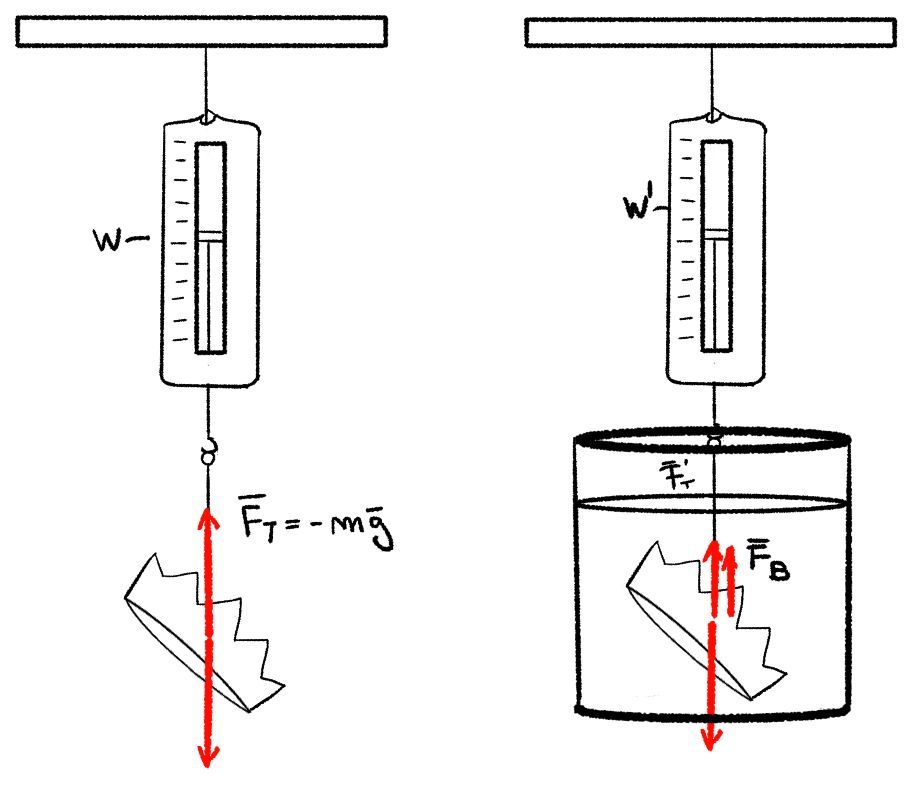
\includegraphics[height=2.2in]{images/arquimedes.jpg}
    \caption{Exercise \theexample }
    \label{4}
  \end{center}
\end{figure}

% Fifth Section %%%%%%%%%%%%%%%%%%%%%%%%%%%%%%%%%%%%%%%%%%%%
\stepcounter{example}

\section*{Exercise \theexample}


Helium balloon. What volume $V$ of helium is needed if a balloon is to lift a load of $180~kg$ (including the weight of the empty balloon)?


\begin{figure}[h!]
  \begin{center}
    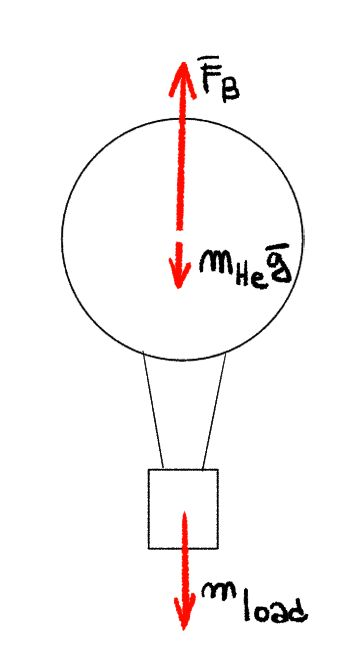
\includegraphics[height=2.7in]{images/baloom.jpg}
    \caption{Exercise \theexample }
    \label{5}
  \end{center}
\end{figure}



% Fifth Section %%%%%%%%%%%%%%%%%%%%%%%%%%%%%%%%%%%%%%%%%%%%
\stepcounter{example}

\section*{Exercise \theexample}

Suppose a piece of styrofoam, $\rho=180~kg/m^3$ is
held completely submerged in water. (a) What is the
tension in the cord? Find this using Archimedes’s principle.
(b) Use $p=p_0+\rho g h$ to calculate directly the force exerted by
the water on the two sloped sides and the bottom of the styrofoam;
then show that the vector sum of these forces is the buoyant
force.

\begin{figure}[h!]
  \begin{center}
  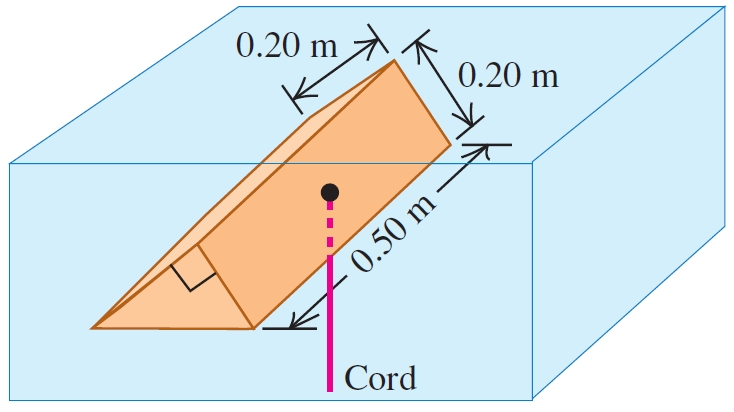
\includegraphics[height=1.5in]{images/example_12.97.jpg}
  \caption{Exercise \theexample }
  \label{6}
\end{center}
\end{figure}



\end{document}


